\documentclass{scrartcl}

\usepackage{eurosym}
\usepackage[utf8]{inputenc}
\usepackage[ngerman]{babel}
\usepackage{verbatim}
\usepackage{graphicx}
\usepackage{rotating}


\title{Effiziente Graphenalgorithmen - 4. Übung}
\author{Matthias Bady (210235131)\\ Christian Hildebrandt (210238835)\\ Sven Mertke (210235818)}

\begin{document}

\maketitle
%{{{
\section{Aufgabe 4.1}
%}}}
Ja, bidirektionale und zielgerichtete Suche lassen sich sinnvoll kombinieren. Der Algorithmus erfolgt analog dem bidirektionalen Dijkstra, der ebenfalls zielgerichtet, bidirektional arbeitet. Einzige Bedingung, die an den Algorithmus zu stellen ist, ist dass er den gleichen Weg vom Start zum Zielknoten und vice versa findet - also korrekt arbeitet.
%{{{
\section{Aufgabe 4.2}
%}}}
\subsection*{Ansatz 1}
Da das asymptotische Verhalten untersucht werden soll, wird angenommen, jeder Knoten in D verfügt über jeweils K Nachfolger. Da es sich bei D um einen bipartiten Graph handelt, befinden sich diese K Nachfolger jeweils in der konträren Menge. Weiterhin soll angenommen werden, das jeder Pfad in D aus T Kanten besteht. Ausgehend vom Startknoten s enthält eine Menge damit $\sum_{i=1}^{T}{K^i}$ Knoten und die andere Menge $\sum_{i=1}^{T-1}{K^i}$ Knoten. Der Startknoten wird wegen der asymptotischen Betrachtung vernachlässigt. Damit ist die Gesamtzahl der Knoten in D und die Zahl der äußeren Iterationen $\sum_{i=1}^{T}{K^i}$. Allerdings ist die Kantenliste im letzten Durchlauf leer, so daß die Komplexität hier bei $O(K^T*0)$ liegt. Insgesamt liegt diese also bei $O((1+\sum_{i=1}^{T}{K^i} - K^T)*m) = O((\sum_{i=1}^{T-1}{K^i})*m)$. Da $\sum_{i=1}^{T-1}{K^i} \leq \sum_{i=1}^{T}{K^i}$ gilt $O(n_1*m)$

\subsection*{Ansatz 2}
Für einen bipartiten Graphen $D=(V_1 \cup V_2, A)$ und $n_1=|V_1|, n_2=|V_2|$ wird maximaler Knotengrad angenommen. Es wird dann in 2 Fälle unterschieden:
\\\\
\textbf{untere Grenze (minimaler Graph) $V_1 < V_2$:}
Ausgehend vom Startknoten $S \in V_1$ verlaufen bei maximalem Knotengrad $n_2$ Kanten zu $n_2$ Knoten aus $V_2$. Hier ist \mbox{$|S|=n_1=1, m=|V_2|=n_2$} und somit der zeitliche Aufwand $O(n_{1}m)$
\\\\
\textbf{obere Grenze (maximaler Graph) $V_1 = V_2$:}
Widerum ausgehend von $S \in V_1$ verlaufen genau $n_2$ Kanten nach $V_2$ und von $V_2$ aus maximal $n_1*n_2$ Kanten nach $V_1$. Die Queue beinhaltet dann $S+n_2+n_1$ Knoten, wobei für alle $n_1$ Knoten außer $S$ keine neuen Kanten betrachtet werden müssen, da diese bereits bei der Abarbeitung aller Knoten aus $V_2$ erfasst wurden. Die Laufzeit betragt daher für $n_1=n_2$ \mbox{$O(1+n_2*m+n_1*0)=O(n_{1}m)$}.

\subsection*{Ansatz 3}

Sei $D= \left( V_{1} \cup V_{2}, A \right)$ ein bipartiter Graph, mit $n_{1} = \vert V_{1} \vert$, $n_{1} = \vert V_{1} \vert$ und $n_{1} \leq n_{2}$. Sei $s \in V$ der Startknoten der kürzesten Wege von $s$ nach $v \in V$ und sei $d(v)$ die Länge des kürzesten $s$-$v$-Weges, dann beträgt $d(v)$ für beliebige $v \in V$ in einem bipartiten Graphen $D$ höchstens $2 \min \left( n_{1}, n_{2} \right) + 1 = 2n_{1} + 1$. Demnach benötigt der Algorithmus höchstens $2n_{1} + 1$ Durchläufe und mit jeweils $O(m)$ Zeit pro Durchlauf, ergibt sich eine Gesamtlaufzeit von $O(n_{1}m)$.

%{{{
\section{Aufgabe 4.3}
%}}}
\begin{description}
\item[a)]
\end{description}
Sei $c_{ij}^{k}$ die Länge der Kante $(i,j)$ im $k$-ten Durchlauf und sei $T_{k}$ der Kürzeste-Wege-Baum. Für beliebige $(i,j) \in T_{k-1}$ gilt, $d_{k-1}^{*} (j) = d_{k-1}^{*} (i) + c_{ij}^{k-1}$. Aus $c_{ij}^{k} \leq 2c_{ij}^{k-1} + 1$, $\forall (i,j) \in A$ erhält man $2d_{k-1}^{*} (i) + c_{ij}^{k} - 2d_{k-1}{*} (j) \leq 1$, $\forall (i,j) \in T_{k-1}$. Definiert man die in $P_{k}$ reduzierten Kantenlängen hinsichtlich der Distanzen $d_{k-1}^{*}$, dann hat jede Kante in $T_{k-1}$ eine Länge von höchstens $1$. Es gibt also einen gerichteten Pfad von $s$ zu jeden anderen Knoten dessen reduzierte Kantenlänge höchstens $n$ beträgt.

\begin{description}
\item[b)]
\end{description}
Die reduzierten Kantenlängen hinsichtlich der Distanzen $d_{k-1}^{*}$ sind alle nichtnegativ. Damit kann Dijkstra  zur Lösung des Kürzeste-Wege-Problems in $P_{k}$ verwendet werden. Jeder kürzeste Weg hat eine Länge von höchstens $n$ und unter Benutzung der Dial's-Variante des Dijkstra, folgt eine Laufzeit von $O(m)$. Die Operationen \verb+decreaseKey+ und \verb+findMin+ laufen in $O(1)$ und im $k$-ten Schritt kann ein kürzester Pfad von $u$ nach $v$ in $O(m)$ gefunden werden. Demnach gilt für den Bitscaling-Algorithmus eine Gesamtlaufzeit von $O(km) = O(m \log C)$, mit $C = \max_{(u,v) \in A} \lbrace c(u,v) \rbrace$.
\newpage
%{{{
\section{Aufgabe 4.4}
%}}}
\begin{center}
\begin{figure}[h]
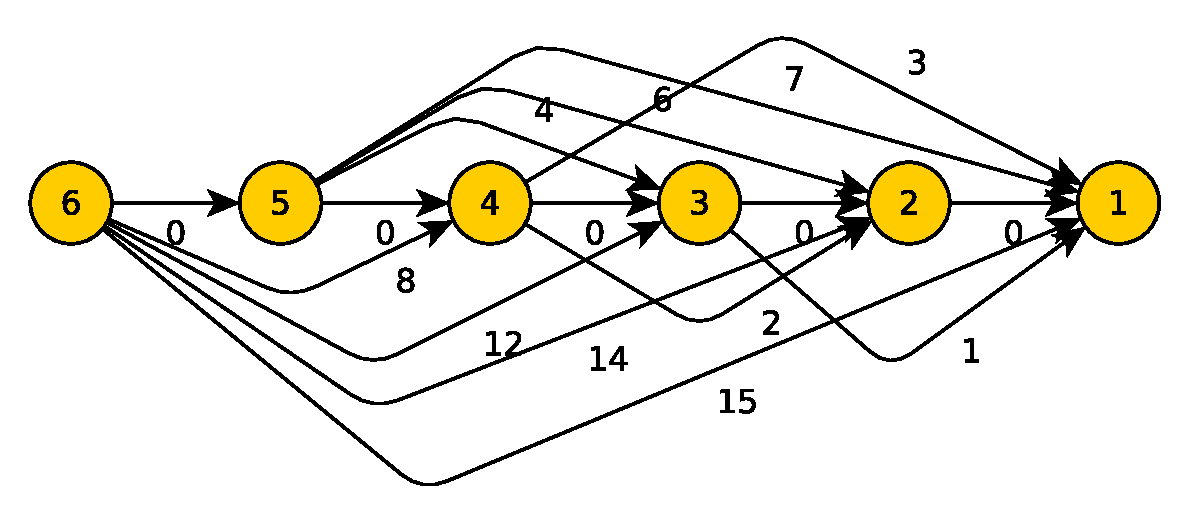
\includegraphics[scale=0.7]{effGra_4_4-1.eps}
\caption{Graph für $n=6$}
\end{figure}
\end{center}

\begin{table}[h]
  \centering

       \begin{tabular}{cr}
          Knoten          &Adj.-Liste\\
          \hline\hline
          1       &6\, 5\, 4\, 3\, 2\\
          2       &6\, 5\, 4\, 3\, 1\\
          3       &6\, 5\, 4\, 2\, 1\\
          4       &6\, 5\, 3\, 2\, 1\\
          5       &6\, 4\, 3\, 2\, 1\\
          6       &1\, 2\, 3\, 4\, 5\\
        \end{tabular}
  \caption{Adjazenzlisten}
  \label{tab:adjlis}
\end{table}


\begin{table}[h]
       \begin{tabular}{c|cccccc|rc}
          Iteration & Label 1 & Label 2 & Label 3 & Label 4 & Label 5 & Label 6 & Schritt & Pfad\\
          \hline\hline
          0       & $\infty$ & $\infty$ & $\infty$ & $\infty$ & $\infty$ & 0 & init & $\emptyset$\\
          $\vdots$       & $\vdots$ & $\vdots$ & $\vdots$ & $\vdots$ & $\vdots$ & $\vdots$ & Relax 6 & $\vdots$\\
          5       & 15 & 14 & 12 & 8 & 0 & 0 & Relax 6 & 6-1\\
          6       & 14 & 14 & 12 & 8 & 0 & 0 & Relax 2 & 6-2-1\\
          $\vdots$       & $\vdots$ & $\vdots$ & $\vdots$ & $\vdots$ & $\vdots$ & $\vdots$ & Relax 2 & $\vdots$\\
          9       & 13 & 14 & 12 & 8 & 0 & 0 & Relax 3 & 6-3-1\\
          $\vdots$       & $\vdots$ & $\vdots$ & $\vdots$ & $\vdots$ & $\vdots$ & $\vdots$ & Relax 3 & $\vdots$\\
          11       & 12 & 12 & 12 & 8 & 0 & 0 & Update 3-2 & 6-3-2-1\\
          $\vdots$       & $\vdots$ & $\vdots$ & $\vdots$ & $\vdots$ & $\vdots$ & $\vdots$ & Update & $\vdots$\\
          14       & 11 & 12 & 12 & 8 & 0 & 0 & Relax 4 & 6-4-1\\
          $\vdots$       & $\vdots$ & $\vdots$ & $\vdots$ & $\vdots$ & $\vdots$ & $\vdots$ & Relax 4 & $\vdots$\\
          18       & 10 & 10 & 12 & 8 & 0 & 0 & Update 4-2 & 6-4-2-1\\
          19       & 9 & 10 & 8 & 8 & 0 & 0 & Update 4-3 & 6-4-3-1\\
          $\vdots$       & $\vdots$ & $\vdots$ & $\vdots$ & $\vdots$ & $\vdots$ & $\vdots$ & Update & $\vdots$\\
          21       & 8 & 10 & 8 & 8 & 0 & 0 & Update 4-3-2 & 6-4-3-2-1\\
          $\vdots$       & $\vdots$ & $\vdots$ & $\vdots$ & $\vdots$ & $\vdots$ & $\vdots$ & Update & $\vdots$\\
          25       & 7 & 10 & 8 & 8 & 0 & 0 & Relax 5 & 6-5-1\\
          $\vdots$       & $\vdots$ & $\vdots$ & $\vdots$ & $\vdots$ & $\vdots$ & $\vdots$ & Relax 5 & $\vdots$\\
          27       & 6 & 6 & 8 & 8 & 0 & 0 & Update 5-2 & 6-5-2-1\\
          $\vdots$       & $\vdots$ & $\vdots$ & $\vdots$ & $\vdots$ & $\vdots$ & $\vdots$ & Update & $\vdots$\\
          29       & 5 & 6 & 4 & 8 & 0 & 0 & Update 5-3 & 6-5-3-1\\
          30       & 4 & 6 & 4 & 8 & 0 & 0 & Update 5-3-2 & 6-5-3-2-1\\
          $\vdots$       & $\vdots$ & $\vdots$ & $\vdots$ & $\vdots$ & $\vdots$ & $\vdots$ & Update & $\vdots$\\
          33       & 3 & 6 & 4 & 0 & 0 & 0 & Update 5-4 & 6-5-4-1\\
          $\vdots$       & $\vdots$ & $\vdots$ & $\vdots$ & $\vdots$ & $\vdots$ & $\vdots$ & Update & $\vdots$\\
          36       & 2 & 2 & 4 & 0 & 0 & 0 & Update 5-4-2 & 6-5-4-2-1\\
          $\vdots$       & $\vdots$ & $\vdots$ & $\vdots$ & $\vdots$ & $\vdots$ & $\vdots$ & Update & $\vdots$\\
          39       & 1 & 2 & 0 & 0 & 0 & 0 & Update 5-4-3 & 6-5-4-3-1\\
          $\vdots$       & $\vdots$ & $\vdots$ & $\vdots$ & $\vdots$ & $\vdots$ & $\vdots$ & Update & $\vdots$\\
          42       & 0 & 0 & 0 & 0 & 0 & 0 & Update 5-4-3-2 & 6-5-4-3-2-1\\
       \end{tabular}
  \caption{Ablauf Dequeue Implementierung Label-Correcting Algorithm}
  \label{tab:alg}
\end{table}


\end{document}